%
% This is the LaTeX template file for lecture notes for CS294-8,
% Computational Biology for Computer Scientists.  When preparing 
% LaTeX notes for this class, please use this template.
%
% To familiarize yourself with this template, the body contains
% some examples of its use.  Look them over.  Then you can
% run LaTeX on this file.  After you have LaTeXed this file then
% you can look over the result either by printing it out with
% dvips or using xdvi.
%
% This template is based on the template for Prof. Sinclair's CS 270.

\documentclass[twoside]{ctexart}

\usepackage{listings,xcolor}
\usepackage{enumitem}
\usepackage{mathrsfs}
\usepackage{indentfirst} 
\usepackage{lstcustom}
\usepackage{ctex}
\usepackage{comment}
\usepackage{booktabs}
\usepackage{graphicx}
\usepackage{diagbox}
\usepackage{amsmath,amsfonts,graphicx,amssymb,bm,amsthm}
\usepackage{algorithm,algorithmicx}
\usepackage[noend]{algpseudocode}
\usepackage{fancyhdr}
\usepackage{tikz}
\usepackage{graphicx}
\usetikzlibrary{arrows,automata}
\usepackage{hyperref}

\setlength{\oddsidemargin}{0.25 in}
\setlength{\evensidemargin}{0.25 in}
\setlength{\topmargin}{-0.6 in}
\setlength{\textwidth}{6.5 in}
\setlength{\textheight}{8.5 in}
\setlength{\headsep}{0.75 in}
\setlength{\parindent}{0 in}
\setlength{\parskip}{0.1 in}

%
% The following commands set up the lecnum (lecture number)
% counter and make various numbering schemes work relative
% to the lecture number.
%
\newcounter{lecnum}
\newcounter{counter_exm}\setcounter{counter_exm}{1}
\newtheorem{theorem}{\hskip 1.7em 定理}
\newtheorem{lemma}[theorem]{\hskip 1.7em 引理}
\newtheorem{proposition}[theorem]{Proposition}
\newtheorem{claim}[theorem]{\hskip 1.7em 命题}
\newtheorem{corollary}[theorem]{\hskip 1.7em 推论}
\newtheorem{definition}[theorem]{\hskip 1.7em 定义}

\renewcommand{\emph}[1]{\begin{kaishu}#1\end{kaishu}}

\newenvironment{solution}{{\noindent\hskip 2em \bf 解 \quad}}


\renewenvironment{proof}{{\noindent\hskip 2em \bf 证明 \quad}}{\hfill$\qed$\par}
\newenvironment{example}{{\noindent\hskip 2em \bf 例 \arabic{counter_exm}\quad}}{\addtocounter{counter_exm}{1}\par}

\newenvironment{concept}[1]{{\bf #1\quad} \begin{kaishu}} {\end{kaishu}\par}

\newcommand\E{\mathbb{E}}

%
% The following macro is used to generate the header.
%

\newcommand{\lecture}[4]{
   \pagestyle{myheadings}
   \thispagestyle{plain}
   \newpage
   \setcounter{lecnum}{#1}
   \setcounter{page}{1}
   \noindent
   \begin{center}
   \framebox{
      \vbox{\vspace{2mm}
    \hbox to 6.28in { {\bf 计算机系统导论小班
                        \hfill 2020年秋季} }
       \vspace{4mm}
       \hbox to 6.28in { {\Large \hfill 课程回顾#1:#2  \hfill} }
       \vspace{2mm} 
       \hbox to 6.28in { {\it  \hfill 作者:#3} }
      \vspace{2mm}}
   }
   \end{center}
   \markboth{课程回顾#1:#2}{课程回顾#1:#2}
   {\bf 免责声明}:{\it 该笔记尚未进行正式出版物的通常审查,未经教师允许不能向课程外分发.}
   \vspace*{4mm}
}


\renewcommand{\cite}[1]{[#1]}
\def\beginrefs{\begin{list}%
        {[\arabic{equation}]}{\usecounter{equation}
         \setlength{\leftmargin}{2.0truecm}\setlength{\labelsep}{0.4truecm}%
         \setlength{\labelwidth}{1.6truecm}}}
\def\endrefs{\end{list}}
\def\bibentry#1{\item[\hbox{[#1]}]}

%Use this command for a figure; it puts a figure in wherever you want it.
%usage: \fig{NUMBER}{SPACE-IN-INCHES}{CAPTION}
\newcommand{\fig}[3]{
			\vspace{#2}
			\begin{center}
			图 \thelecnum.#1:~#3
			\end{center}
	}

% **** IF YOU WANT TO DEFINE ADDITIONAL MACROS FOR YOURSELF, PUT THEM HERE:
\DeclareMathOperator*{\argmax}{\arg\max}
\DeclareMathOperator*{\argmin}{\arg\min}

\begin{document}

% title 
\lecture{1}{Bits and Bytes/Integers}{杨晨阳}


    
    \section{信息存储}

    \subsection{字节和存储}
    \begin{enumerate}
        \item    对于一个字长w位的机器而言,可表示的虚拟地址有[0, $2^{w} - 1$]。
        \item 基本C数据类型的典型大小:注意long和指针在32位程序里占4个byte,在64位程序里占8个byte。
        \item 多字节的程序对象的排列方式
            \begin{itemize}
            \item 小端法(little endian):最低位的地址值最大,常见于 Sun, PPC Mac, Internet系统
            \item 大端法(big endian):最低位的地址值最小,常见于x86, ARM processors running Android, iOS, Windows系统
            \end{itemize}
            
          注意,字符串与数组的存储顺序与大(小)端法无关!
          
          \begin{figure}[htb]
            \centering
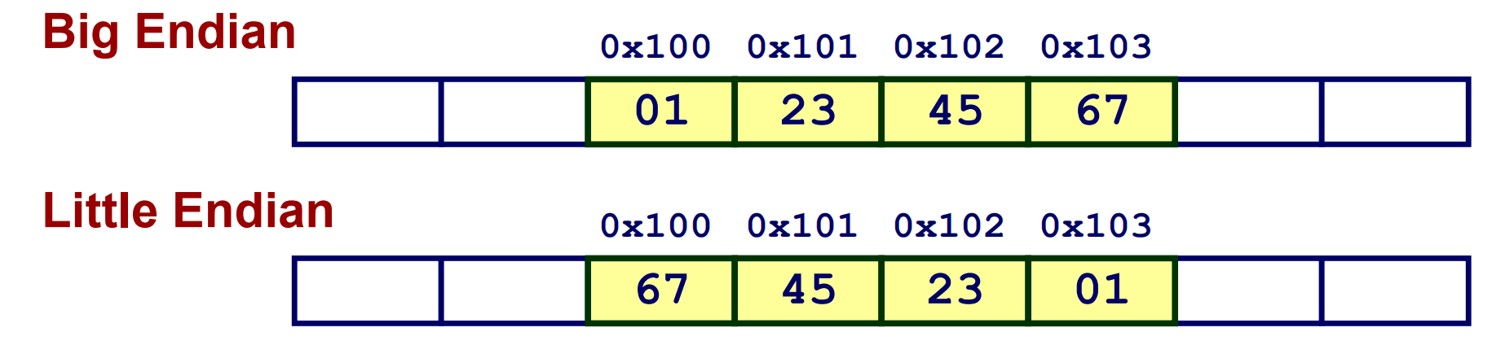
\includegraphics[width = 0.6\textwidth]{figure/Lec1-endian.jpg}
            \caption{大端法/小端法}
            \label{fig:my_label}
        \end{figure}
    \item C语言中字符串被编码为结尾为null字符的字符数组;以最常见的ASCII码为例,每个字符都有一个唯一的十六进制表示,终止字节表示为0x00。

    \end{enumerate}  
    
    
    \subsection{布尔代数}
    % $\sim$,  $ \wedge{}$, $ \&$,  | 的运算法则
    
    \begin{itemize}
        \item And:两个运算数都为1时,结果为1
        \item Or:两个运算数有一个为1时,结果为1
        \item Not:一元运算符,把0变成1,把1变成0
        \item Xor:两个运算数相同时为0,否则为1。(即布尔环上的加法)
    \end{itemize}
    可以将运算符扩展到对位向量的运算。
    
    \subsection{逻辑运算}
    逻辑运算符||, $\&\&$, !,分别对应命题逻辑中的或,与,非。所有非零参数都表示TRUE,0表示FALSE。
    

    位运算和逻辑运算的区别:
    \begin{itemize}
        \item 位级运算一定会把整个式子算完;逻辑运算不一定会把整个式子算完,如果第一个参数求值后能确定表达式结果,则会提前结束。(即短路求值)
        \item 位级运算得到的结果是位向量,逻辑运算得到的结果是1(True)或者0(False)。
    \end{itemize}
    \subsection{移位运算}
    \begin{itemize}
        \item 左移:x << k, 即x向左移动k位,丢到最高的k位,并在右端补上k个0
        \item 右移:逻辑右移在左端补上k个0,算术右移在左端补上k个最高有效位的值。
    \end{itemize}
    无符号数的右移一定是逻辑右移;有符号数的右移几乎在所有编译器/机器组合中都是算术右移。
    
    注意:
    \begin{enumerate}
        \item 
    移动的位数应$\ge0$ 且 $<w$,以免造成未知错误。取模的行为并没有\textbf{保证}。
    \item 要注意运算的优先级,不确定时最好加括号,以免造成错误。例如:$1<<2+3<<4$。 \textbf{注意:}加减法的优先级高于移位的优先级。
    \item 算术右移作用于有符号数x后相当于$x/2^k$(向下取整)。注意,C语言中直接使用表达式$x/2^k$是向零取整。
    \end{enumerate}

    \section{整数表示}

    \subsection{无符号数和有符号数的对比}
    \begin{enumerate}
        \item 表达方式:无符号数直接按数学方法转化为二进制,有符号数使用补码。两者唯一区别在于最高位的权重不同,无符号数权重为$2^{w-1}$,有符号数权重为$-2^{w-1}$。
        \item 表示范围:无符号数为$[0,2^{w}-1]$,有符号数为$[-2^{w-1},2^{w-1}-1]$。
        
        以32位整数为例,UMin=0的十六进制为$0x00000000$,UMax$=2^w-1$的十六进制为0xFFFFFFFF,TMin$=-2^{w-1}$的十六进制为$0x80000000$,TMax$=2^{w-1}-1$的十六进制为 0x7FFFFFFF,-1的十六进制为0xFFFFFFFF。
        
        \item 转换:由于两者只是最高位权重有差别,因此在最高位为0时,两者表达的值相同;在最高位为1时,无符号数表达的值比有符号数大$2^w=2^{w-1}+2^{w-1}$。
        \begin{itemize}
        \item 有符号数转换成相应的无符号数:负数变成较大的正数,非负数保持不变。
        \item 无符号数转换成相应的有符号数:较大的正数变成负数,较小的非负数保持不变。
    \end{itemize}
    注:转换过程中,\textbf{位模式不变,解读方式不同},得到的数值可能不同。
        
    \end{enumerate}

    \subsection{其它}
    \begin{enumerate}
        \item 
    C语言中:当执行一个运算时,一个运算数有符号,另一个无符号,则\textbf{将有符号数隐式转换为无符号数},并假设均为非负,再进行计算。
    \item 扩展(用来完成从一个较小的数据类型转换到一个较大的类型):
    \begin{itemize}
        \item 无符号数:零扩展,在前面加0
        \item 有符号数:符号扩展,在前面加符号位
    \end{itemize}
    \item 截断:
    直接将该数字截断为所需要的位数,再按所需要的方式解读即可。
    \end{enumerate}
    
	\section{整数运算}
	注意:无论是无符号数还是有符号数,整数运算都直接对对应位模式进行,并将运算结果对$2^w$取模,最后按所需的方式解读即可。
	\subsection{加法溢出}
	无符号数当且仅当和小于其中一个加数时,发生了溢出。有符号数中,两加数均为正且结果为负或者两加数为负且结果为正,为溢出。
	
	\subsection{整数减法}
	$-x = \sim x + 1$。(观察对应的位模式,$\sim x + x=$0xFFFFFFFF,$+1$后恰为零元),	因此整数减法可以转为整数加法进行考虑。
	\subsection{整数乘法}
	乘以常数:编译器倾向于用移位和加减法结合来减小运算所需的代价。
	
	\subsection{整数除法}
	舍入:整数除法总是舍入到0,对正数来说是向下舍入,对负数来说是向上舍入。
	计算$x/2^{w}$时,根据x的类型:
	\begin{itemize}
	    \item 无符号除法:直接将x右移k位
	    \item 有符号除法:在$x<0$时,对$x + (1 << k) - 1$右移k位,在$x\ge 0$时,直接对$x$右移k位。($x<0$时向上舍入的推导请参考课本)
	\end{itemize}
\end{document}




